%LTeX: language=it
\subsubsection{UC 5 - Creazione di un evento nel calendario} \label{sec:UC5}
    \begin{itemize}
        \item \textbf{Attore principale}: MUA;
        \item \textbf{Descrizione}: il MUA crea un evento nel calendario del sistema;
        \item \textbf{Precondizioni}: il MUA sta usando la funzionalità di creazione di un oggetto;
        \item \textbf{Postcondizioni}: il sistema salva il nuovo evento nel calendario di sistema;
        \item \textbf{Scenario principale}:
            \begin{enumerate}
                \item il MUA invia i dati per creare il nuovo evento nel calendario (\hyperref[sec:UC5.1]{UC 5.1});
                \item il sistema elabora le informazioni ricevute;
                \item il sistema salva l'evento nel calendario;
            \end{enumerate}
        \item \textbf{Inclusioni}: nessuna;
        \item \textbf{Generalizzazioni}: nessuna;
        \item \textbf{Estensioni}: nessuna.
    \end{itemize}

\begin{figure}[h]
    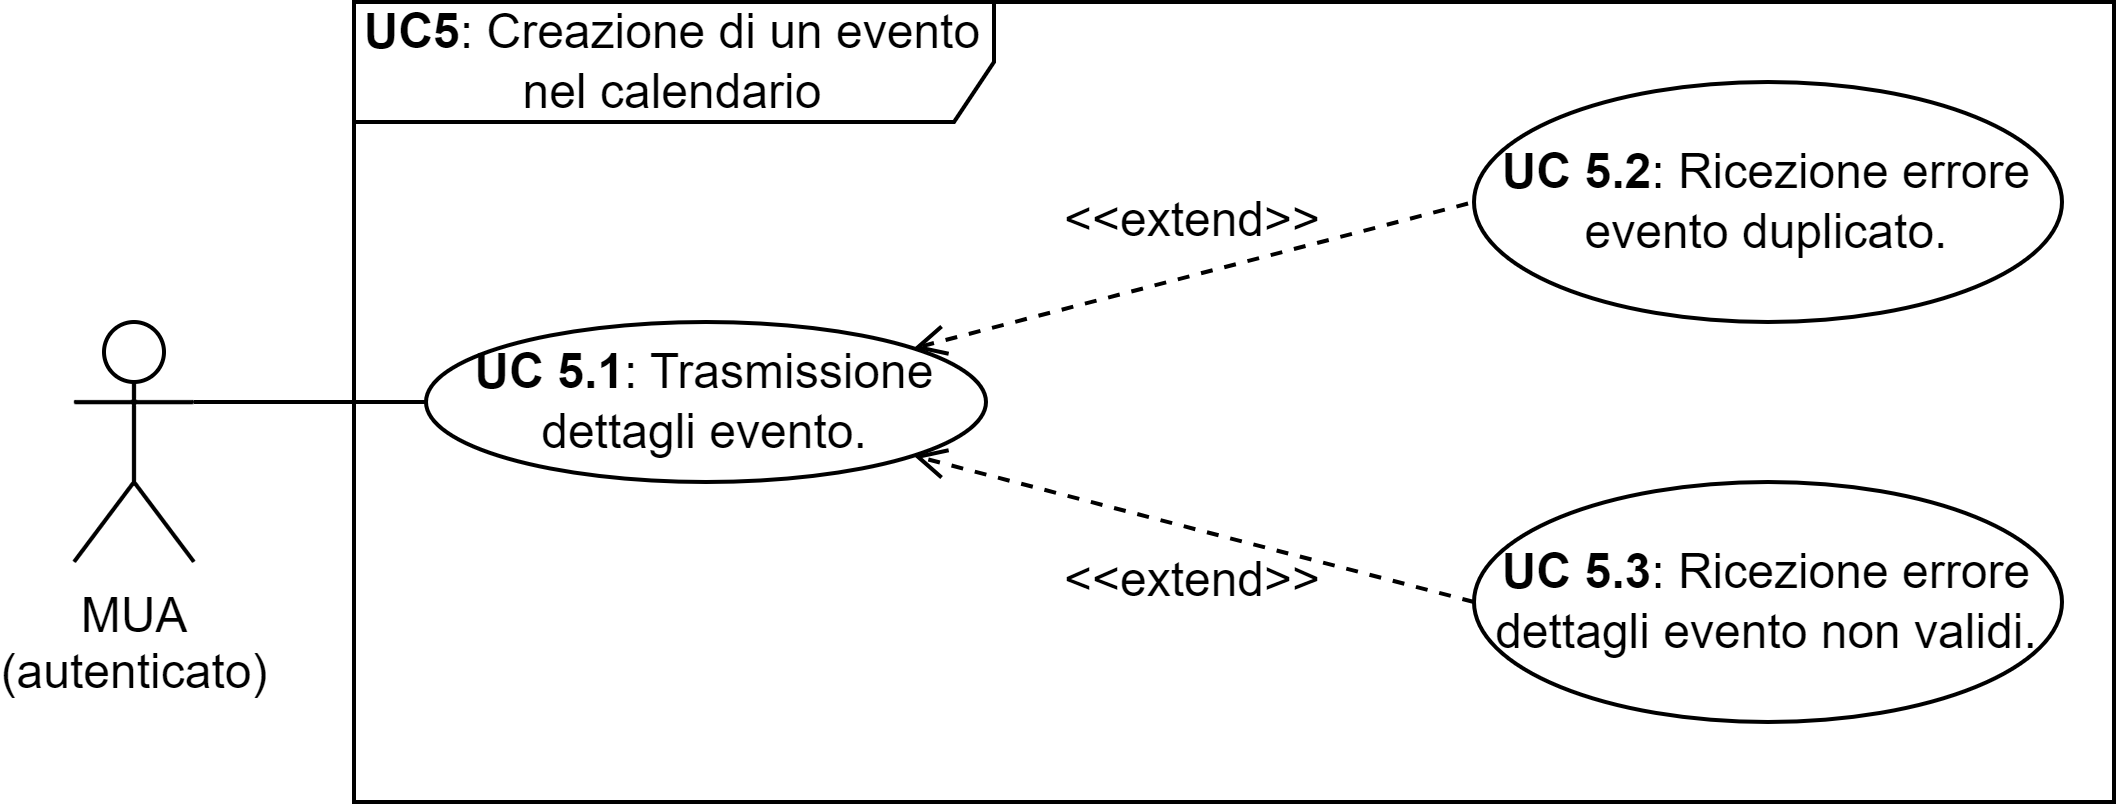
\includegraphics[width=0.85\textwidth]{sections/uc_imgs/UC05.X.png}
    \centering
    \caption{Diagramma sotto-casi UC 5.}
\end{figure}

\subsubsection{UC 5.1 - Trasmette i dettagli dell'evento} \label{sec:UC5.1}
    \begin{itemize}
        \item \textbf{Attore principale}: MUA;
        \item \textbf{Descrizione}: il MUA crea un evento nel calendario del sistema;
        \item \textbf{Precondizioni}: il MUA sta usando la funzionalità di creazione di un oggetto;
        \item \textbf{Postcondizioni}: il sistema salva il nuovo evento nel calendario di sistema;
        \item \textbf{Scenario principale}:
            \begin{enumerate}
                \item il MUA invia i dati per creare il nuovo evento nel calendario;
                \item il sistema elabora le informazioni ricevute;
                \item il sistema salva l'evento nel calendario;
            \end{enumerate}
        \item \textbf{Inclusioni}: nessuna;
        \item \textbf{Generalizzazioni}: nessuna;
        \item \textbf{Estensioni}:
            \begin{enumerate}[label=\alph*.]
                \item il sistema non riesce a salvare l'evento nel calendario perché è un duplicato:
                \begin{enumerate}[label=\arabic*.]
                    \item il sistema ritorna un errore al MUA di evento duplicato (\hyperref[sec:UC5.2]{UC 5.2});
                \end{enumerate}
                \item il sistema non riesce a salvare l'evento nel calendario perché i dettagli inviati sono errati:
                \begin{enumerate}[label=\arabic*.]
                    \item il sistema ritorna un errore al MUA che le informazioni fornite sono errate (\hyperref[sec:UC5.3]{UC 5.3}).
                \end{enumerate}
            \end{enumerate}
    \end{itemize}

\subsubsection{UC 5.2 - Ricezione errore evento duplicato} \label{sec:UC5.2}
    \begin{figure}[h]
        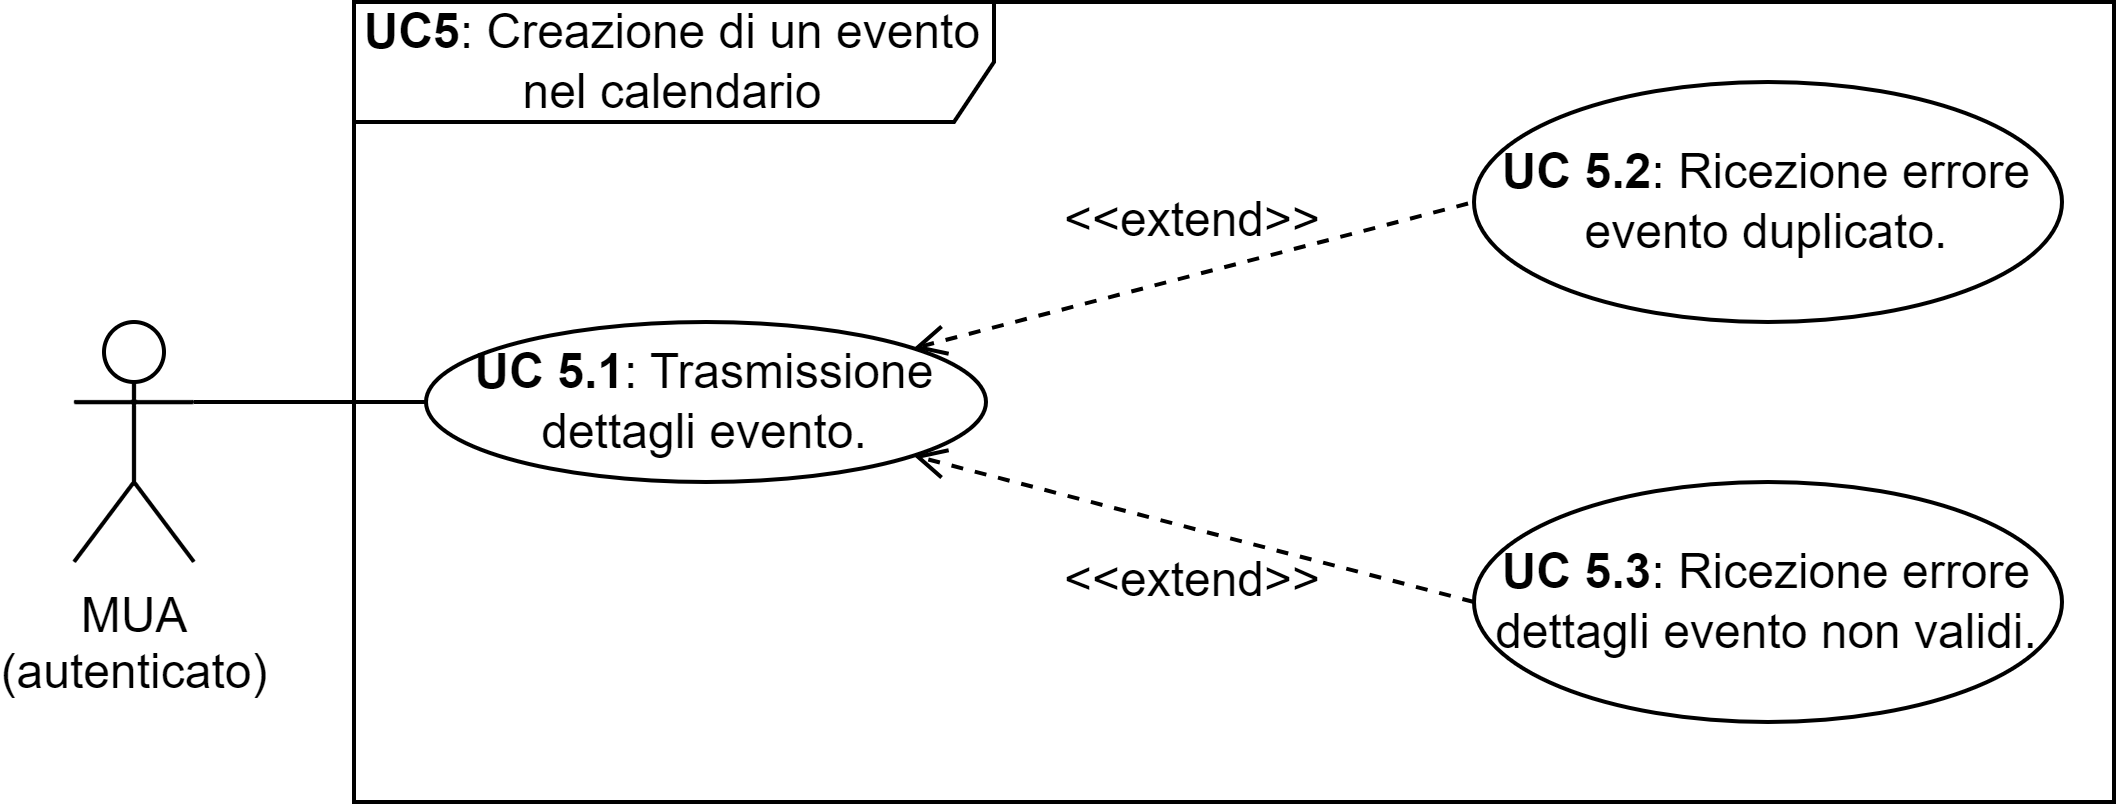
\includegraphics[width=0.85\textwidth]{sections/uc_imgs/UC05.X.png}
        \centering
        \caption{Diagramma UC 5.}
    \end{figure}
    \begin{itemize}
        \item \textbf{Attore principale}: MUA;
        \item \textbf{Descrizione}: il MUA crea un evento nel calendario del sistema;
        \item \textbf{Precondizioni}: il MUA sta usando la funzionalità di creazione di un oggetto;
        \item \textbf{Postcondizioni}: il sistema salva il nuovo evento nel calendario di sistema;
        \item \textbf{Scenario principale}:
            \begin{enumerate}
                \item il MUA invia i dati per creare il nuovo evento nel calendario;
                \item il sistema elabora le informazioni ricevute;
                \item il sistema salva l'evento nel calendario;
            \end{enumerate}
        \item \textbf{Inclusioni}: nessuna;
        \item \textbf{Generalizzazioni}: nessuna;
        \item \textbf{Estensioni}:
            \begin{enumerate}[label=\alph*.]
                \item il sistema non riesce a salvare l'evento nel calendario perché è un duplicato:
                \begin{enumerate}[label=\arabic*.]
                    \item il sistema ritorna un errore al MUA di evento duplicato (\hyperref[sec:UC5.1]{UC 5.1});
                \end{enumerate}
                \item il sistema non riesce a salvare l'evento nel calendario perché i dettagli inviati sono errati:
                \begin{enumerate}[label=\arabic*.]
                    \item il sistema ritorna un errore al MUA che le informazioni fornite sono errate (\hyperref[sec:UC5.2]{UC 5.2}).
                \end{enumerate}
            \end{enumerate}
    \end{itemize}

\subsubsection{UC 5.3 - Ricezione errore dettagli evento non validi} \label{sec:UC5.2}
    \begin{figure}[h]
        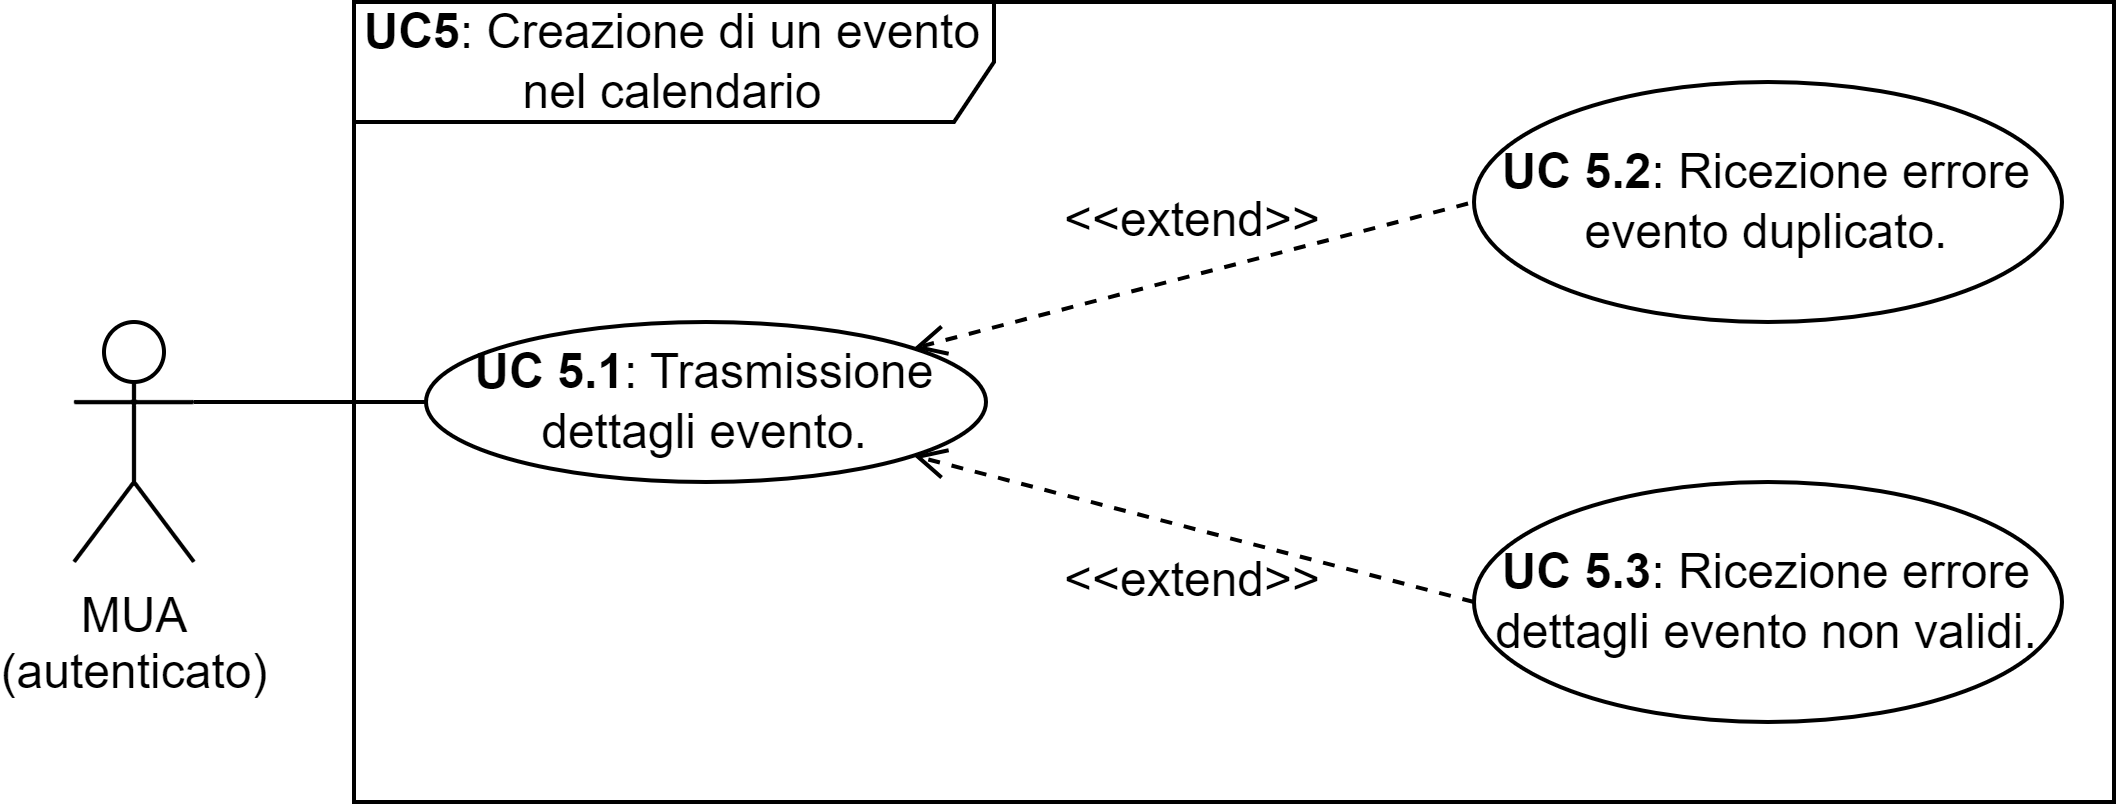
\includegraphics[width=0.85\textwidth]{sections/uc_imgs/UC05.X.png}
        \centering
        \caption{Diagramma UC 5.}
    \end{figure}
    \begin{itemize}
        \item \textbf{Attore principale}: MUA;
        \item \textbf{Descrizione}: il MUA crea un evento nel calendario del sistema;
        \item \textbf{Precondizioni}: il MUA sta usando la funzionalità di creazione di un oggetto;
        \item \textbf{Postcondizioni}: il sistema salva il nuovo evento nel calendario di sistema;
        \item \textbf{Scenario principale}:
            \begin{enumerate}
                \item il MUA invia i dati per creare il nuovo evento nel calendario;
                \item il sistema elabora le informazioni ricevute;
                \item il sistema salva l'evento nel calendario;
            \end{enumerate}
        \item \textbf{Inclusioni}: nessuna;
        \item \textbf{Generalizzazioni}: nessuna;
        \item \textbf{Estensioni}:
            \begin{enumerate}[label=\alph*.]
                \item il sistema non riesce a salvare l'evento nel calendario perché è un duplicato:
                \begin{enumerate}[label=\arabic*.]
                    \item il sistema ritorna un errore al MUA di evento duplicato (\hyperref[sec:UC5.1]{UC 5.1});
                \end{enumerate}
                \item il sistema non riesce a salvare l'evento nel calendario perché i dettagli inviati sono errati:
                \begin{enumerate}[label=\arabic*.]
                    \item il sistema ritorna un errore al MUA che le informazioni fornite sono errate (\hyperref[sec:UC5.2]{UC 5.2}).
                \end{enumerate}
            \end{enumerate}
    \end{itemize}

\subsubsection{UC 6 - Creazione di una cartella} \label{sec:UC6}
    \begin{itemize}
        \item \textbf{Attore principale}: MUA;
        \item \textbf{Descrizione}: il MUA crea una cartella nel sistema;
        \item \textbf{Precondizioni}: il MUA sta usando la funzionalità di creazione di un oggetto;
        \item \textbf{Postcondizioni}: il sistema salva la nuova cartella creata;
        \item \textbf{Scenario principale}:
            \begin{enumerate}
                \item il MUA invia le informazioni per creare la cartella;
                \item il sistema elabora le informazioni ricevute;
                \item il sistema salva la nuova cartella;
            \end{enumerate}
        \item \textbf{Inclusioni}: nessuna;
        \item \textbf{Generalizzazioni}: nessuna;
        \item \textbf{Estensioni}:
            \begin{enumerate}[label=\alph*.]
                \item il sistema non riesce a salvare la cartella perché è un duplicato:
                \begin{enumerate}[label=\arabic*.]
                    \item il sistema ritorna un errore al MUA di cartella duplicata (\hyperref[sec:UC3.9]{UC 3.9});
                \end{enumerate}
                \item il sistema non riesce a creare la cartella perché l'account che sta eseguendo l'azione non ha i premessi necessari:
                \begin{enumerate}[label=\arabic*.]
                    \item il sistema ritorna un errore al MUA che l'account che sta eseguendo l'azione non ha i privilegi neccessari per farla (\hyperref[sec:UC3.10]{UC 3.10}).
                \end{enumerate}
            \end{enumerate}
    \end{itemize}